% Intended LaTeX compiler: xelatex
\documentclass[12pt]{spbstu-task}
\usepackage{graphicx}
\usepackage{float}
\usepackage{booktabs}
\usepackage{dsfont}
\usepackage{hyperref}
\setmainfont{Times New Roman}
\defaultfontfeatures{Ligatures=TeX,Scale=MatchLowercase,Mapping=tex-text}
\hypersetup{hidelinks}
\allowdisplaybreaks
\captionsetup[table]{labelsep=period}
\captionsetup[figure]{labelsep=period}
\setlength{\abovecaptionskip}{5pt}
\setlength{\belowcaptionskip}{0pt}
\newcommand{\E}{\mathbb{E}}
\newcommand{\D}{\mathbb{D}}
\renewcommand{\Prob}{\mathbf{P}}
\newcommand{\ind}{\mathds{1}}
\newcommand{\Xm}{\mathbf{X}}
\begin{document}

\sloppy
\pagenumbering{arabic}

\noindent\textbf{Салимли Айзек Мухтар оглы}\hfill\textbf{гр. 5140201/60301}

\begin{center}
  \textbf{ИДЗ №3 (Регрессионный анализ)}\\[0.4em]
  \textbf{Вариант 16}
\end{center}

\noindent\textbf{Задание:}

\begin{center}
  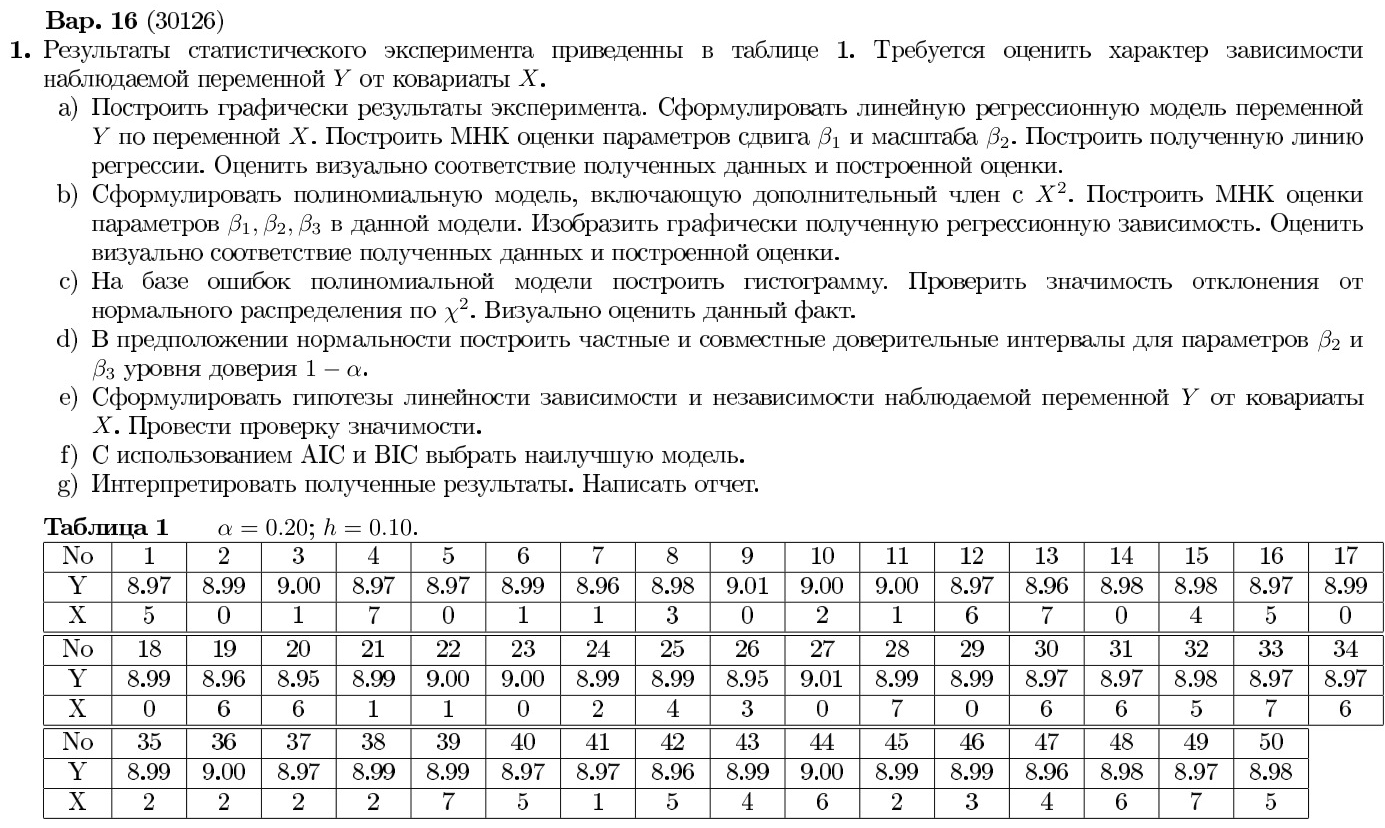
\includegraphics[width=\textwidth]{fig/task.png}
\end{center}

%% Пункт a
\subsection*{1a. Линейная регрессионная модель}
\textbf{Модель:}
\begin{displaymath}
  Y_i = \beta_1 + \beta_2 X_i + \varepsilon_i,\qquad i = 1, \ldots, n,\quad n = 50,
\end{displaymath}
где \(\varepsilon_i\) независимы, \(\E\varepsilon_i = 0\), \(\D\varepsilon_i = \sigma^2\); \(\beta_1\) - параметр сдвига,
\(\beta_2\) - параметр масштаба. В матричной форме \(Y = \Xm^{\mathsf{T}}\beta + \varepsilon\), где
\(\beta = (\beta_1, \beta_2)^{\mathsf{T}}\), а \(\Xm\) - матрица размера \(2\times n\), в которой первая строка
из единиц отвечает за сдвиг \(\beta_1\), а вторая содержит наблюдаемые значения ковариаты:
\begin{displaymath}
  \Xm = \begin{pmatrix} 1 & 1 & \ldots & 1 \\ X_1 & X_2 & \ldots & X_n \end{pmatrix}.
\end{displaymath}

\textbf{МНК оценки.} Минимизируем сумму квадратов отклонений:
\begin{gather*}
  SS(\beta) = \sum_{i=1}^{n}\left(Y_i - \beta_1 - \beta_2 X_i\right)^2 = \left|Y - \Xm^{\mathsf{T}}\beta\right|^2 \to \min_\beta,\\
  \frac{\partial SS}{\partial\beta} = -2\Xm\left(Y - \Xm^{\mathsf{T}}\beta\right) = 0
  \;\Rightarrow\; \Xm\Xm^{\mathsf{T}}\beta = \Xm Y
  \;\Rightarrow\; \hat{\beta} = B\,\Xm Y,\qquad B = \left(\Xm\Xm^{\mathsf{T}}\right)^{-1}.
\end{gather*}
По данным:
\begin{displaymath}
  \Xm\Xm^{\mathsf{T}} = \begin{pmatrix} n & \sum X_i \\ \sum X_i & \sum X_i^2 \end{pmatrix}
  = \begin{pmatrix} 50 & 166 \\ 166 & 858 \end{pmatrix},\qquad
  \Xm Y = \begin{pmatrix} \sum Y_i \\ \sum X_i Y_i \end{pmatrix} = \begin{pmatrix} 449.06 \\ 1489.93 \end{pmatrix}.
\end{displaymath}
Решение системы в явном виде (\(\bar{X} = 3.32\), \(\bar{Y} = 8.9812\)):
\begin{gather*}
  \hat{\beta}_2 = \frac{\sum_{i=1}^{n}(X_i - \bar{X})(Y_i - \bar{Y})}{\sum_{i=1}^{n}(X_i - \bar{X})^2}
  = \frac{-0.9492}{306.88} = -0.0030931,\\
  \hat{\beta}_1 = \bar{Y} - \hat{\beta}_2\bar{X} = 8.9812 + 0.0030931\cdot 3.32 = 8.99147.
\end{gather*}

\textbf{Остатки и оценка дисперсии:} \(\hat{\varepsilon}_i = Y_i - \hat{\beta}_1 - \hat{\beta}_2 X_i\),
\begin{gather*}
  SSE = \sum_{i=1}^{n}\hat{\varepsilon}_i^2 = 0.0081921,\\
  s^2 = \frac{SSE}{n - 2} = 1.7067\cdot 10^{-4}\quad(\text{несмещенная оценка } \sigma^2),\qquad s = 0.013064,\\
  B = \begin{pmatrix} 0.055918 & -0.010819 \\ -0.010819 & 0.0032586 \end{pmatrix},\qquad
  \widehat{\D\hat{\beta}} = s^2B,\\
  \sqrt{s^2B_{11}} = 0.003089,\qquad \sqrt{s^2B_{22}} = 0.000746.
\end{gather*}

\begin{center}
  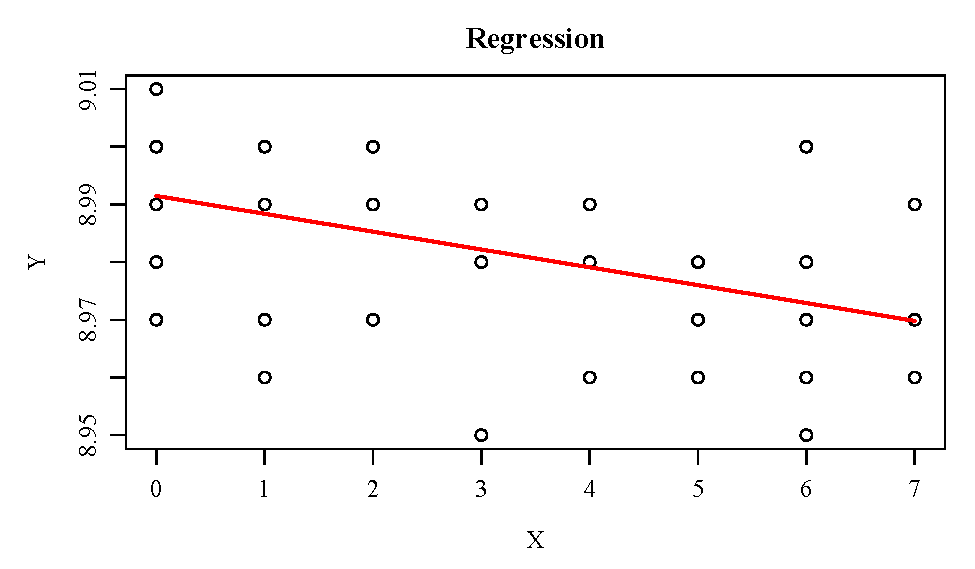
\includegraphics[width=0.92\textwidth]{fig/t1a_lin.pdf}
\end{center}

Прямая \(\hat{Y} = 8.99147 - 0.0030931X\) убывает: от 8.9915 при \(X = 0\) до 8.9698 при \(X = 7\). Это изменение
(0.022) того же порядка, что и разброс точек вокруг прямой (\(s = 0.013\)), поэтому зависимость слабая.
Многие точки совпадают, так как \(X\) целые, а \(Y\) записан с точностью 0.01. При \(X = 5, 6, 7\) точки уже
почти не опускаются, прямая это не отражает.

\noindent\textbf{Вывод:} \(\hat{\beta}_1 = 8.99147\), \(\hat{\beta}_2 = -0.0030931\), \(s^2 = 1.7067\cdot 10^{-4}\).

%% Пункт b
\subsection*{1b. Полиномиальная модель}
\textbf{Модель:}
\begin{displaymath}
  Y_i = \beta_1 + \beta_2 X_i + \beta_3 X_i^2 + \varepsilon_i,\qquad i = 1, \ldots, n,\qquad
  \Xm = \begin{pmatrix} 1 & \ldots & 1 \\ X_1 & \ldots & X_n \\ X_1^2 & \ldots & X_n^2 \end{pmatrix}\ (3\times n).
\end{displaymath}
МНК оценка находится так же: \(\hat{\beta} = B\,\Xm Y\), \(B = \left(\Xm\Xm^{\mathsf{T}}\right)^{-1}\):
\begin{gather*}
  \Xm\Xm^{\mathsf{T}} = \begin{pmatrix} n & \sum X_i & \sum X_i^2 \\ \sum X_i & \sum X_i^2 & \sum X_i^3 \\
    \sum X_i^2 & \sum X_i^3 & \sum X_i^4 \end{pmatrix}
  = \begin{pmatrix} 50 & 166 & 858 \\ 166 & 858 & 4936 \\ 858 & 4936 & 29910 \end{pmatrix},\\
  \Xm Y = \begin{pmatrix} \sum Y_i \\ \sum X_i Y_i \\ \sum X_i^2 Y_i \end{pmatrix}
  = \begin{pmatrix} 449.06 \\ 1489.93 \\ 7699.75 \end{pmatrix},\\
  B = \begin{pmatrix} 0.085695 & -0.048168 & 0.0054908 \\ -0.048168 & 0.050105 & -0.0068871 \\
    0.0054908 & -0.0068871 & 0.0010125 \end{pmatrix},\qquad
  \hat{\beta} = B\,\Xm Y = \begin{pmatrix} 8.99332 \\ -0.0054139 \\ 0.00034120 \end{pmatrix}.
\end{gather*}
Остатки \(\hat{\varepsilon}_i = Y_i - \hat{\beta}_1 - \hat{\beta}_2 X_i - \hat{\beta}_3 X_i^2\) и оценка дисперсии:
\begin{gather*}
  SSE = 0.0080771,\qquad s^2 = \frac{SSE}{n - 3} = 1.7185\cdot 10^{-4},\qquad s = 0.013109,\\
  \sqrt{s^2B_{11}} = 0.0038376,\qquad \sqrt{s^2B_{22}} = 0.0029344,\qquad \sqrt{s^2B_{33}} = 0.00041713.
\end{gather*}

\begin{center}
  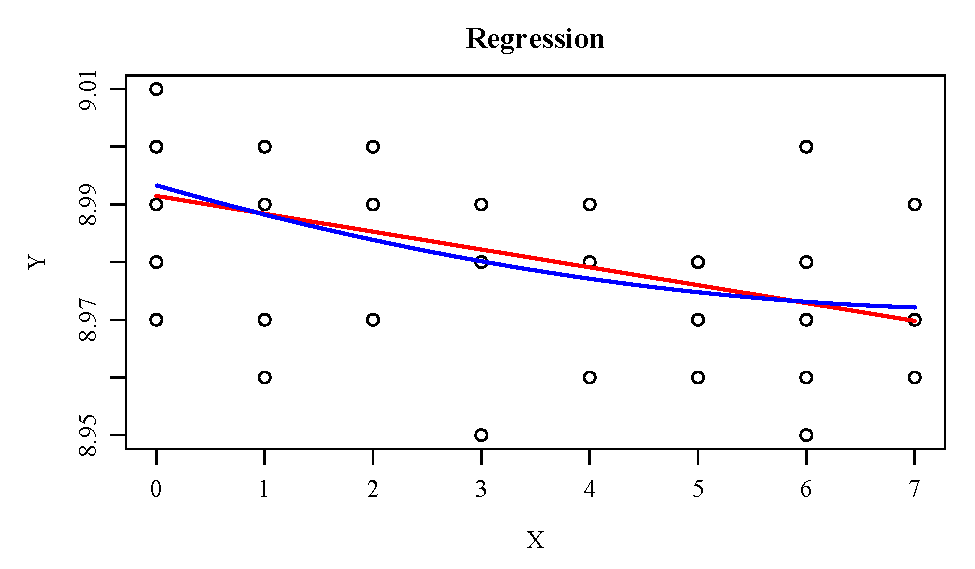
\includegraphics[width=0.92\textwidth]{fig/t1b_poly.pdf}
\end{center}

Парабола \(\hat{Y} = 8.99332 - 0.0054139X + 0.00034120X^2\) выпуклая вниз (\(\hat{\beta}_3 > 0\)), ее вершина
\(X = -\hat{\beta}_2/(2\hat{\beta}_3) = 7.93\) лежит правее данных. Поэтому на \([0;\ 7]\) кривая убывает, но все
медленнее, и при \(X = 6, 7\) почти не меняется, что лучше согласуется с точками справа. От прямой она отличается мало: \(SSE\) уменьшилась только с 0.0081921 до 0.0080771.

\noindent\textbf{Вывод:} \(\hat{\beta}_1 = 8.99332\), \(\hat{\beta}_2 = -0.0054139\), \(\hat{\beta}_3 = 0.00034120\),
\(s^2 = 1.7185\cdot 10^{-4}\).

%% Пункт c
\subsection*{1c. Анализ ошибок полиномиальной модели}
Ошибки модели оцениваем остатками \(\hat{\varepsilon}_i\) из пункта 1b и считаем их независимыми.
Остатки лежат в \([-0.03015;\ 0.02688]\), размах 0.057. Шаг \(h = 0.10\) из таблицы 1 больше размаха, при нем
все остатки попали бы в один интервал, поэтому гистограмма построена со стандартным шагом 0.01
(это и точность записи \(Y\)).

\begin{center}
  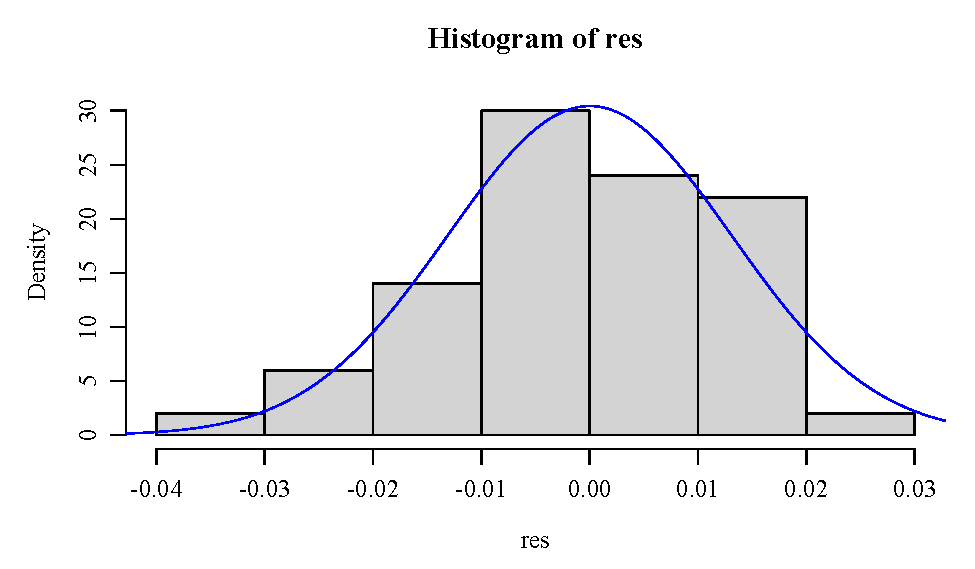
\includegraphics[width=0.92\textwidth]{fig/t1c_hist.pdf}
\end{center}

Для визуального сравнения на графике построена плотность нормального распределения \(\mathcal{N}(0, s^2)\)
с оценкой \(s = 0.013109\) из пункта 1b.

\textbf{Гипотеза} (сложная, неизвестен один параметр \(\sigma\); среднее равно 0 по модели):
\begin{displaymath}
  H_0:\ \varepsilon_i \sim \mathcal{N}(0, \sigma^2)\ \text{при некотором}\ \sigma > 0;\qquad
  H_1:\ \text{распределение ошибок не нормальное}.
\end{displaymath}
Объединяем крайние интервалы гистограммы так, чтобы ожидаемые частоты были не меньше 5, и продолжаем крайние
интервалы до \(\pm\infty\): получаем \(r = 4\) интервала \((-\infty;\ -0.01]\), \((-0.01;\ 0]\), \((0;\ 0.01]\),
\((0.01;\ +\infty)\) с частотами \(\nu_i = 11, 15, 12, 12\). Вероятности и статистика:
\begin{displaymath}
  p_i(\sigma) = \Phi\left(\frac{u_i}{\sigma}\right) - \Phi\left(\frac{l_i}{\sigma}\right),\qquad
  X^2(\sigma) = \sum_{i=1}^{r}\frac{\left(\nu_i - np_i(\sigma)\right)^2}{np_i(\sigma)},
\end{displaymath}
где \(\Phi\) - функция распределения \(\mathcal{N}(0, 1)\). Так как подставлять в \(X^2\) оценку \(s\) по
негруппированным остаткам нельзя, \(\sigma\) оцениваем по сгруппированным данным.

\textbf{Минимизируем хи-квадрат:}
\begin{gather*}
  \hat{X}^2 = \min_{\sigma > 0} X^2(\sigma),\qquad
  \frac{dX^2}{d\sigma} = -\sum_{i=1}^{r}\frac{\nu_i^2}{np_i^2(\sigma)}\frac{dp_i}{d\sigma} = 0,\\
  \frac{dp_i}{d\sigma} = -\frac{z_i\Phi'(z_i) - z_{i-1}\Phi'(z_{i-1})}{\sigma},\qquad
  z_i = \frac{u_i}{\sigma}\quad(z_0 = -\infty,\ z_r = +\infty),\\
  \Phi'(z) = \frac{1}{\sqrt{2\pi}}e^{-z^2/2}.
\end{gather*}
Уравнение явно не решается, поэтому минимум ищем численно градиентным спуском по этой производной, начиная
с \(\sigma = s = 0.013109\):
\begin{displaymath}
  \sigma^{\text{нов}} = \sigma - \eta\,\frac{dX^2}{d\sigma}(\sigma).
\end{displaymath}
Если на очередном шаге \(X^2\) выросла, шаг \(\eta\) делим пополам; останавливаемся, когда
\(\left|dX^2/d\sigma\right| < 10^{-8}\). Понадобилось 12 итераций, перебор по сетке дает ту же точку:
\begin{displaymath}
  \tilde{\sigma} = 0.013496,\qquad \hat{X}^2 = X^2(\tilde{\sigma}) = 0.3765.
\end{displaymath}
При \(H_0\) \(\hat{X}^2 \xrightarrow{d} \chi^2_{r - 1 - k}\), где \(k = 1\) - число оцениваемых параметров,
т.е. \(df = 4 - 1 - 1 = 2\).

\begin{table}[H]
  \caption{Критерий \(\chi^2\) для ошибок при \(\tilde{\sigma} = 0.013496\)}
  \centering
  \small
  \setlength{\tabcolsep}{2pt}
  \begin{tabularx}{\textwidth}{c*{7}{Y}}
    \toprule
    \(i\) & \(l_i\):\newline нижняя граница & \(u_i\):\newline верхняя граница & \(\nu_i\):\newline наблюдаемые
    & \(p_i(\tilde{\sigma})\):\newline вероятности & \(np_i(\tilde{\sigma})\):\newline ожидаемые
    & \(\frac{\nu_i - np_i}{\sqrt{np_i}}\):\newline остатки & \(\frac{(\nu_i - np_i)^2}{np_i}\):\newline вклад в \(X^2\) \\
    \midrule
    1 & \(-\infty\) & -0.01 & 11 & 0.2294 & 11.468 & -0.1381 & 0.0191 \\
    2 & -0.01 & 0 & 15 & 0.2706 & 13.532 & 0.3990 & 0.1592 \\
    3 & 0 & 0.01 & 12 & 0.2706 & 13.532 & -0.4165 & 0.1735 \\
    4 & 0.01 & \(+\infty\) & 12 & 0.2294 & 11.468 & 0.1572 & 0.0247 \\
    \midrule
    \(\sum\) & & & 50 & 1 & 50 & & 0.3765 \\
    \bottomrule
  \end{tabularx}
\end{table}

Критерий (\(df = 2\), граница 3.2189 - квантиль уровня \(1 - \alpha = 0.8\) распределения \(\chi^2_2\)):
\begin{gather*}
  \varphi(X) =
  \begin{cases}
    1, & \hat{X}^2 > 3.2189,\\
    0, & \hat{X}^2 \le 3.2189,
  \end{cases}\\
  \hat{X}^2 = 0.3765 \le 3.2189 \;\Rightarrow\; \varphi(X) = 0,\qquad
  p\text{-value} = \Prob\left(\chi^2_2 > 0.3765\right) = 0.8284,\\
  x_\alpha = 3.2189.
\end{gather*}

\noindent\textbf{Вывод:} принимается \(H_0:\ \varepsilon_i \sim \mathcal{N}(0, \sigma^2)\) на уровне \(\alpha = 0.20\),
\(\alpha_{\max} = 0.8284\); визуально гистограмма с этим согласуется.

%% Пункт d
\subsection*{1d. Частные доверительные интервалы для \(\beta_2\) и \(\beta_3\)}
В предположении нормальности \(\hat{\beta} \sim \mathcal{N}\left(\beta, \sigma^2B\right)\),
\((n - 3)s^2/\sigma^2 \sim \chi^2_{n - 3}\), и они независимы, поэтому
\begin{displaymath}
  \frac{\hat{\beta}_j - \beta_j}{\sqrt{s^2B_{jj}}} \sim S_{n - 3},\qquad j = 2, 3,
\end{displaymath}
где \(S_{n - 3}\) - функция распределения Стьюдента с \(n - 3\) степенями свободы. Отсюда
\begin{gather*}
  \Prob\left(\left|\frac{\hat{\beta}_j - \beta_j}{\sqrt{s^2B_{jj}}}\right| \le x_\alpha\right) = 1 - \alpha,\qquad
  x_\alpha = S^{-1}_{n - 3}\left(1 - \frac{\alpha}{2}\right) = S^{-1}_{47}(0.9) = 1.2998,\\
  \beta_j \in \left[\hat{\beta}_j - d_j;\ \hat{\beta}_j + d_j\right],\qquad d_j = x_\alpha\sqrt{s^2B_{jj}}.
\end{gather*}
По данным (\(1 - \alpha = 0.8\)):
\begin{gather*}
  d_2 = 1.2998\cdot 0.0029344 = 0.0038142,\\
  \beta_2 \in [-0.0054139 - 0.0038142;\ -0.0054139 + 0.0038142] = [-0.0092282;\ -0.0015997],\\
  d_3 = 1.2998\cdot 0.00041713 = 0.00054220,\\
  \beta_3 \in [0.00034120 - 0.00054220;\ 0.00034120 + 0.00054220] = [-0.00020100;\ 0.00088340].
\end{gather*}
Интервал для \(\beta_2\) целиком отрицательный, а интервал для \(\beta_3\) содержит 0.

\noindent\textbf{Вывод} (уровень доверия 0.8):
\begin{itemize}[label=\textbullet]
  \item \(\beta_2 \in [-0.0092282;\ -0.0015997]\);
  \item \(\beta_3 \in [-0.00020100;\ 0.00088340]\).
\end{itemize}
\end{document}
